% Introduction
% Numbers come from reports/results_table.md, reports/ablation.csv and the other sections.

\section{Introduction}
\label{sec:intro}

Once a wildfire is burning, the question that matters for the next day is where it will spread.
Knowing which areas are likely to burn helps crews and resources be placed ahead of the fire front.
Physics-based simulators answer this from fuel, weather and terrain~\cite{rothermel1972}, but they need
detailed fuel descriptions and are not fitted to observed fires. Satellites now record active fires
daily, so the question can also be posed as a learning problem: given today's fire and conditions,
predict tomorrow's fire.

We study this problem on the Next Day Wildfire Spread (NDWS) dataset of Huot
et al.~\cite{huot2022}. It contains 18\,545 samples over the contiguous United States from 2012 to
2020, each a $64\times64$\,km patch at 1\,km resolution. The authors call them fire events, but one
fire can appear in several overlapping samples (Section~\ref{sec:events}). Each patch has 12 inputs on day $t$ (the active
fire mask plus weather, drought, vegetation, terrain and population) and the fire mask on day $t+1$ as
the label. Two properties make the task hard. First, it is extremely imbalanced: only 1.1\% of labelled
training pixels burn the next day, so a model that never predicts fire is already more than 98\%
accurate. Second, the signal is spatial: a pixel's own weather says little about whether it will
burn, while nearby fire and wind direction say a great deal. In the dataset paper, a convolutional
network that sees the whole patch clearly beats pixel models that see only a pixel and its eight
neighbours, and later U-Net and transformer models report higher scores still
(Section~\ref{sec:related}).

Phase~1 of our project asks how far classical machine learning can go when it is given the right
spatial information. We keep a per-pixel model, which is fast to train and easy to inspect, and move
the spatial reasoning into engineered features. Gradient-boosted trees then learn from these features.
Fig.~\ref{fig:pipeline} shows the pipeline. Our contributions are:

\begin{figure*}[t]
\centering
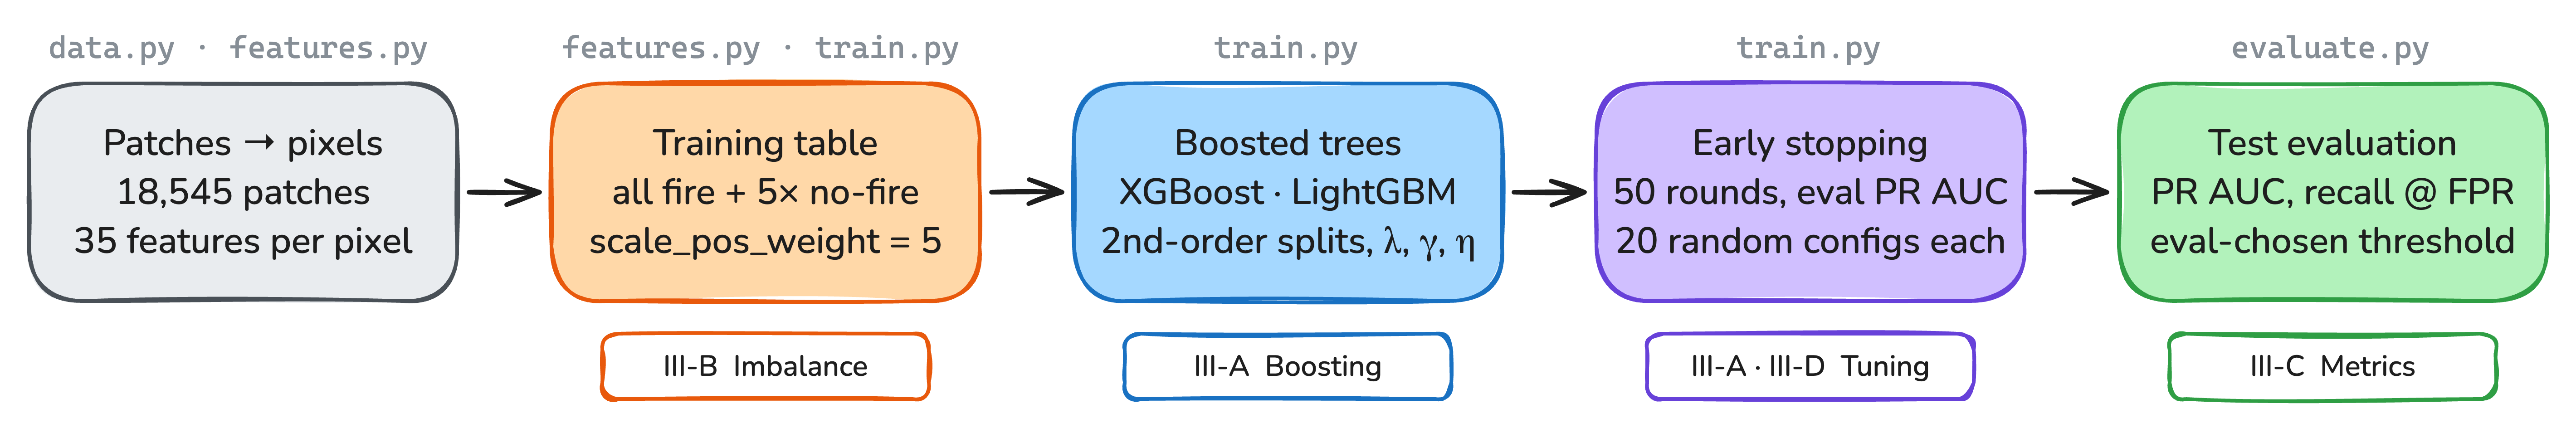
\includegraphics[width=\textwidth]{figures/th_pipeline.png}
\caption{Our Phase~1 pipeline (\texttt{src/}). Each tag names the part of Section~\ref{sec:theory} that
explains that step.}
\label{fig:pipeline}
\end{figure*}
\begin{itemize}
\item a TensorFlow-free data pipeline with physical clipping of export artefacts, and the finding that
the patches are stored south-up, which every direction-dependent feature relies on;
\item 23 engineered features in five groups, including fire density at three scales, distance to the
nearest fire, fire upwind at up to 8\,km, and vapour pressure deficit;
\item tuned XGBoost and LightGBM models whose test PR AUC (0.257 and 0.248) lies between the dataset
authors' pixel models and their CNN;
\item an analysis of what the model learns and where it fails: a feature-group ablation, SHAP values,
a downwind plausibility check, error analysis and an evaluation by fire event.
\end{itemize}

Section~\ref{sec:related} reviews related work, and Section~\ref{sec:theory} gives the theory behind
our modelling choices. The following sections describe the dataset and exploratory analysis, the
methodology and feature engineering, and the results. The last section concludes and outlines
Phase~2.
